% Created 2016-08-17 Wed 14:38
\documentclass[tikz]{standalone}

\usepackage[utf8]{inputenc}
\usepackage[T1]{fontenc}
\usepackage{helvet}
\usepackage{../../templates/msc}

\renewcommand{\familydefault}{\sfdefault}

\tikzset{
every picture/.style={
line width=1pt
}}

\usepackage{tikz}
\author{Holger Karl}
\date{\today}
\title{}


\usetikzlibrary{positioning, fit} 


\begin{document}
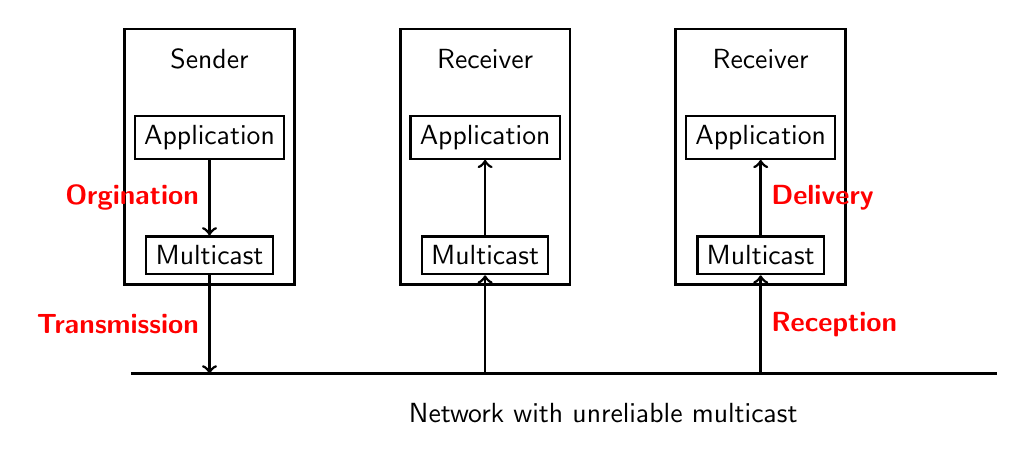
\begin{tikzpicture}[auto, 
block/.style = {rectangle, draw=black, thick, align=left},
node distance = 1cm]

\begin{scope}[on grid]

  \node[block] (s_app) at (0,3) {Application};
  \node[block] (s_mcast) [on grid, below=1.5 of s_app]  {Multicast};
  \node[block] (r1_app) [on grid, right=3.5cm of s_app]  {Application};
  \node[block] (r1_mcast) [on grid, below=1.5 of r1_app]  {Multicast};
  \node[block] (r2_app) [on grid, right=3.5cm of r1_app]  {Application};
  \node[block] (r2_mcast) [on grid, below=1.5 of r2_app]  {Multicast};

  \draw[thick] (-1,0) --   (10,0) node (network) {};
  \node at (5, -0.5) {Network with unreliable multicast};

  \node (sender) [on grid, above=of s_app] {Sender}; 
  \node (r1) [on grid, above=of r1_app] {Receiver}; 
  \node (r2) [on grid, above=of r2_app] {Receiver}; 

  \node [draw, fit=(s_app) (s_mcast) (sender) ] {}; 
  \node [draw, fit=(r1_app) (r1_mcast) (r1) ] {}; 
  \node [draw, fit=(r2_app) (r2_mcast) (r2) ] {}; 

  \draw [->](s_mcast) -> (s_mcast |- network)  node [left,midway, text=red] {\textbf{Transmission}}; 
  \draw [<-] (r1_mcast) -> (r1_mcast |- network) ;  
  \draw [<-] (r2_mcast) -> (r2_mcast |- network) node [right,midway, text=red] {\textbf{Reception}}; 

  \draw [->](s_app) -> (s_mcast)  node [left,midway, text=red] {\textbf{Orgination}}; 
  \draw [->] (r1_mcast) -> (r1_app) ;  
  \draw [<-] (r2_app) -> (r2_mcast) node [right,midway, text=red] {\textbf{Delivery}}; 
  
\end{scope}
\end{tikzpicture}
\end{document}